\documentclass[a4paper,11pt]{article}
\usepackage[utf8x]{inputenc}
\usepackage[cm]{fullpage}
\usepackage{comment}
\usepackage{graphicx}

%opening
\title{475 - Advanced Topics in Software Engineering \\ Acme Telecom}
\author{Ramie Al-Omari \texttt{ra808}, Dan Cooke \texttt{dc408}, Jonathan Evans \texttt{je08}, Javad Moghisi \texttt{jm308}}

\begin{document}
\maketitle

Our client requested a minor modification to a simple, but vital mobile phone customer billing system; the current charging criteria charges customers peak rate for the entire duration of their call if any part of the call falls within a peak period. New regulations stipulate calls must be charged at peak rate only for the time spent within a peak period. This report examines our approaches and techniques used to safely modify and enhance the existing legacy codebase.

We quickly learned there was no documentation present (formal, tests or code comments). This presented us with a major problem; an unknown existing system specification. The requirements specified that other than the stipulated modification, all other functionality should remain unchanged. Clearly the existing functionality would need to be accurately specified to ensure this condition is met. Thus our first goal was to develop a clear specification of the existing system, to allow us to safely refactor the codebase.

We began by implementing a Runner class with a main method to exercise various functionality within the system. The initial workload was split between the group into writing acceptance tests using the FitNesse framework, writing integration tests with JUnit and setting up a developer workflow including build and dependency management as well as a continuous integration server.

We assumed that the deadline for delivering the functionality to comply with the new regulations, coincides with the coursework submission deadline. Therefore our first priority was to ensure that these requirements would be met in a safe and timely manner.


\section{Acceptance Testing}
To specify the functionality of the new system we wrote acceptance tests that captured both the new requirements and the remaining, unchanged behaviour of the old system. As there was no formal specification we had to be careful that these captured the full behaviour of the system. These tests are for testing that the system meets its specification rather than explicitly testing the output of the system (e.g. HTML markup isn't relevant). We specified the following behaviour:

Calls that:
\begin{itemize}
\item start and finish during the same peak time range
\item start and finish during the same off peak time range
\item start during a peak time range and finish at the following off peak time range
\item start during an off peak time range and finish at the following peak time range
\item start during one off peak time range and finish at the following off peak time range
\item start during one peak time range and finish at the following peak time range
\end{itemize}

We implemented the acceptance tests using Fit documents and executed them using the FitNesse acceptance testing framework. We decided to use Fit documents to specify the system as they can easily be edited and read by non-technical stakeholders at AcmeTelecom. FitNesse allows AcmeTelecom to modify, view and run the tests from a user friendly wiki interface. 

Our Fit documents followed the Given When Then structure popular in behaviour driven development. It allowed us to form behaviour "narratives" that used domain language in a natural way that the client can understand. Also most of our tests were data driven and the Given section permitted us to easily specify the information required by the test.  
\\

We established the call charges empirically by running the tests.
\\\\
\begin{tabular}{ l c c }
&				off-peak charges (pence/minute) &  peak charges (pence/minute) \\
business &		0.18&								0.18 \\
leisure & 		0.06& 								0.48 \\
standard & 		0.12&								0.30 \\
\end{tabular}
\\\\


An example of Fit test can be seen below:

\begin{center}
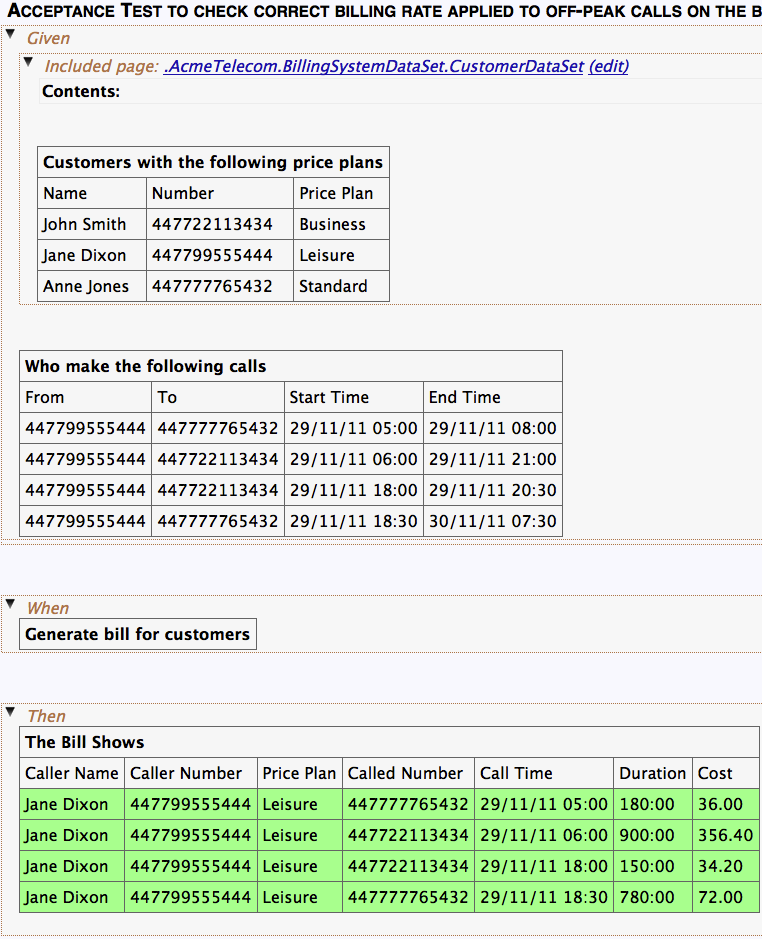
\includegraphics[scale=0.5]{images/fitnesse_test.png}
\end{center}
\pagebreak

\section{Unit Testing}

We implemented a comprehensive passing integration tests to prevent us from breaking existing functionality as we refactored the code base. This was particularly tricky as the createCustomerBills method of BillingSystem output to stdout. The test would set up a number of calls before requesting the bill for those customers. In order to check the output bill we had to redirect Sys.out to a PrintStream, collecting the generated bill into a string on which assertions could be made.

The existing system had not been written with testing in mind so it was very difficult for us to write unit tests or wire up our FitNesse tests. In order to introduce new unit tests we needed to introduce seams enabling us to isolate sections of code. The seams were necessary to break dependencies and allow injection of test values. For example, as the system used the current system time for logging calls, we couldn't create repeatable, non-brittle tests. With the integration tests in place we were confident in refactoring the code to allow arbitrary times to be injected into CallEnd and CallStart.

\begin{verbatim}
public CallEnd(String caller, String callee, long timestamp) {
    super(caller, callee, timestamp);
}
\end{verbatim}

After making these changes we ensured that the integration test continued to pass and started implementing new functionality using Test-Driven Development (TDD).  TDD allows you to be confident your code, helps build up a suite of regression tests and makes your code self documenting. As we broke dependencies we introduced interfaces which could be mocked allowing for testing and verification of object interactions.

Its important to have good code coverage in your test suite with high quality tests which test edge cases to ensure that the tests cover as much of the behaviour of the application as possible. On completion of the task we had 92\% line coverage.

For our unit testing framework we used JUnit assisted by Mockito for mocking objects and EMMA for gathering code coverage statistics. 



\section{Refactoring}

We made heavy use of dependency injection when refactoring the system as it helped us decouple as many classes as possible, making the system more flexible to configuration. We could have gone one step further and used a dependency injection framework such as Google Guice or Spring but this would have only served to make the code harder to refactor and more complex. See http://www.natpryce.com/articles/000783.html. As the codebase is very small the benefits gained would have been small as the object graph of the system is very small and thus easy to hook up. We made interfaces for classes wherever there could be a sensible need to use alternative functionality. Wherever possible we tried to obey the SOLID (Single responsibility, Open closed, Liskob substitution, Interface segregation and Dependency Inversion) principles as they help guide in writing easy to read, extensile and maintainable code. Listed below is some of the refactoring we did.

\begin{itemize}
\item The send method on BillGenerator doesn't actually require totalBill as the line items already have the call cost from which this can calculated so we removed it.
\item Injected BillGenerator into BillingSystem and introduced an interface for it. Its role is to allow for different ways of formatting the bill, for example grouping calls together into peak/off-peak or changing the ordering of the calls.
\item Created a new BillingSystem test which would pass in a mock BillGenerator and verify that its send method is called with the correct arguments. In order to do the verify, equals and hashCode had to be implemented for LineItem Call and CallEvent along with tests.  We noticed that the send method doesn't actually require totalBill as the line items already have the call cost from which this can calculated.
\item We also injected CustomerDatabase and TariffLibrary into the BillingSystem and again used mocking to sense the behaviour. Ports and adapters could have been used to add a layer of abstraction to the CustomerLibrary and Tariff interfaces in case the library changes but we decided against it as the library is maintained internally at Acme Telecom and not third party.
\item Broke up the long createBillForCustomer method into smaller methods such as getCallsForCustomer and calculateCostOfEachCall. 
\item Separated out the logic for calculating call costs into classes which implement a BillCalculator interface.  VariableRateBillCalcuator corresponding to the new, variable billing requirements and FixedRateBillCalculator to the old. If legislation ever changes such that customers need to be billed differently, only a subclass of BillCalculator would have to be added. We only unit tested the VariableRateBillCalculator as the acceptance tests already covered the old fixed rate tariff.
\item The peak period logic hasn't changed and remained in the same place.
\item BillingSystem split into CallLogger and BillingSystem as billing system originally had both roles breaking "Single responsibility" of the S in solid.
\item As the variable tariff is the tariff required for the requirements it is set in the constructor of BillingSystem but it has a setter to override the tariff if required
\item Restructured the system into three packages and removed the cyclic dependency between BillingSystem and BillGenerator (see before diagram).
\item Removed timestamps and replaced them with JodaTime objects which are easier to work with and have a nice descriptive DSL.
\item Implemented nextPeakChange in DaytimePeakPeriod 
\end{itemize}

The code for calculating a bill is greatly simplifed and has been made a lot more readable:
\begin{verbatim}
    private void createBillFor(Customer customer) {
        List<Call> calls = callLogger.getCallsFor(customer);

        Tariff tariff = tariffDatabase.tarriffFor(customer);

        List<LineItem> items = calculateCostOf(calls, tariff);

        billGenerator.send(customer, items);
    }

    private List<LineItem> calculateCostOf(List<Call> calls, Tariff tariff) {
        List<LineItem> items = new ArrayList<LineItem>();

        for (Call call : calls) {
            BigDecimal callCost = billCalculator.getCallCost(call, tariff);
            items.add(new BillItem(call, callCost));
        }
        return items;
}
\end{verbatim}
\pagebreak

Structure before re-factoring:
%Diagram before
\begin{center}
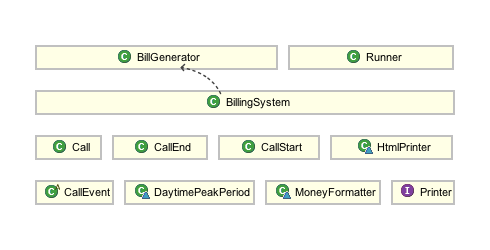
\includegraphics[scale=0.75]{images/original_structure.png}
\end{center}

Structure after re-factoring:
%Diagram after
\begin{center}
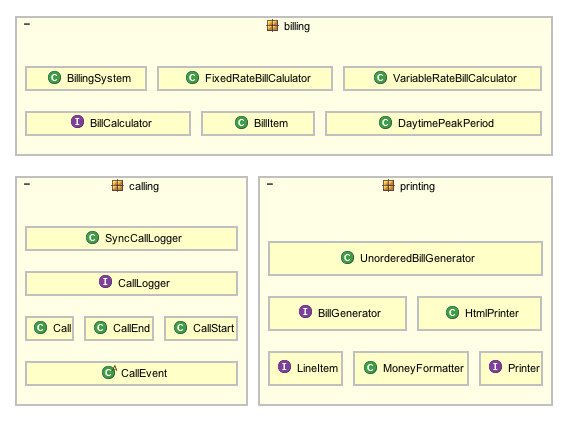
\includegraphics[scale=0.75]{images/new_structure.png}
\end{center}


%Wrote new code
\begin{comment}
\section{Implementing Variable Billing}
As the refactoring has given us an interface "BillCalculator", we can add ng the price can be done in one function, "getCallCost" in the implementation of BillCalculator.

We have decided to make use of Joda-Time for storing call start times and end times, as this class has a lot of useful functions for making calculations with dates.

\begin{verbatim}
public BigDecimal getCallCost(Call call, Tariff tariff, DaytimePeakPeriod peakPeriod) {
    DateTime currentTime = call.startTime();
    DateTime endTime = call.endTime();
    int totalOffPeakDuration = 0;
    int totalPeakDuration = 0;
    while (currentTime.compareTo((call.endTime())) < 0) {
        DateTime nextPeakChange = peakPeriod.nextPeakChange(currentTime);
        int peakDuration = Math.min(Seconds.secondsBetween(currentTime,          endTime).getSeconds(),
        Seconds.secondsBetween(currentTime, nextPeakChange).getSeconds());
        if (peakPeriod.offPeak(currentTime)) {
            totalOffPeakDuration += peakDuration;
        } else {
            totalPeakDuration += peakDuration;
        }
        currentTime = currentTime.plusSeconds(peakDuration);
    }
    BigDecimal offPeakCost = new BigDecimal(totalOffPeakDuration).multiply(tariff.offPeakRate());
    BigDecimal peakCost = new BigDecimal(totalPeakDuration).multiply(tariff.peakRate());
    return offPeakCost.add(peakCost).setScale(0, RoundingMode.HALF_UP);
}
\end{verbatim}

We made us of a new function "nextPeakChange" which given a time, returns the following time boundary between on and off peak. This means we can work out at most how long they should be charged at a given rate in O(1) time.

The code works by starting from the beginning of the call and adding the number of seconds between the current time and the next boundary to either th5e off peak duration or on peak duration. It then continues to do this from the previous boundary until the end. This function has a complexity of O(k) where k is the number of boundaries. As we can assume no conversation lasts over 24 hours, we will only loop at most 3 times.
\end{comment}
\pagebreak

%Anything else you did
\section{Development Process}
We used the GIT distributed version control system to allow our team to effectively collaborate on the same code, hosting our repository on Github as they offer a reliable service and free accounts for students. Using a free micro instance on Amazons Elastic Compute Cloud (EC2) we set up the free Jenkins Continuous Integration (CI) system. Every commit to git would trigger Github's post web hooks, alerting Jenkins that there had been a commit. Jenkins would then checkout the code, build it, run the acceptance tests using FitNesse, integration tests and unit tests using JUnit, and generate code coverage with EMMA. We could also see the status of the builds of all commits along with their code coverage and test status using the Jenkins web interface shown below. Every time the build status changed, i.e. a successful build after a failed build of a failed build after a successful build, and email would be sent to the group as a warning. Using continuous integration enabled the group to track our progress towards a system with full code coverage and then ensure that we maintained the coverage as we made changes. Utilising CI added momentum to the development process as we all wanted full code coverage and to keep the build green. Below is a screenshot of the project page on Jenkins web interface with testing and code coverage graphs.

To manage building and other tasks associated with the project we used Gradle. We used Gradle as it has a good domain model for build tasks and is very flexible, allowing you to use both ant/Maven build tasks and maven repositories if required. Java build targets were set up by simply including the java plugin although we had to add a main class attribute to the jar manifest file. We also used the emma plugin so that every time we built the test task, EMMA code coverage statistics were generated for Jenkins to use. Lastly we used the idea plugin, this allowed us to generate Intellij IDEA project files which had the libraries and build targets as defined in the Maven build. 

When FitNesse tests failed we had to use javas remote debugging from within IntelliJ to attach to the FitNesse process. This allowed is to use all the standard IntelliJ debug tools (breakpoints, stepping through code, variable inspection) to resolve the issue causing the bug.

To deploy the system we would extend the current continuous integration system to automatically promote the new builds to production. As this is a desktop application and not a web app, production could correspond to a versioned folder with a symlink to the latest version (to allow blue/green releasing) or a update system to push the software to the users.
\\\\

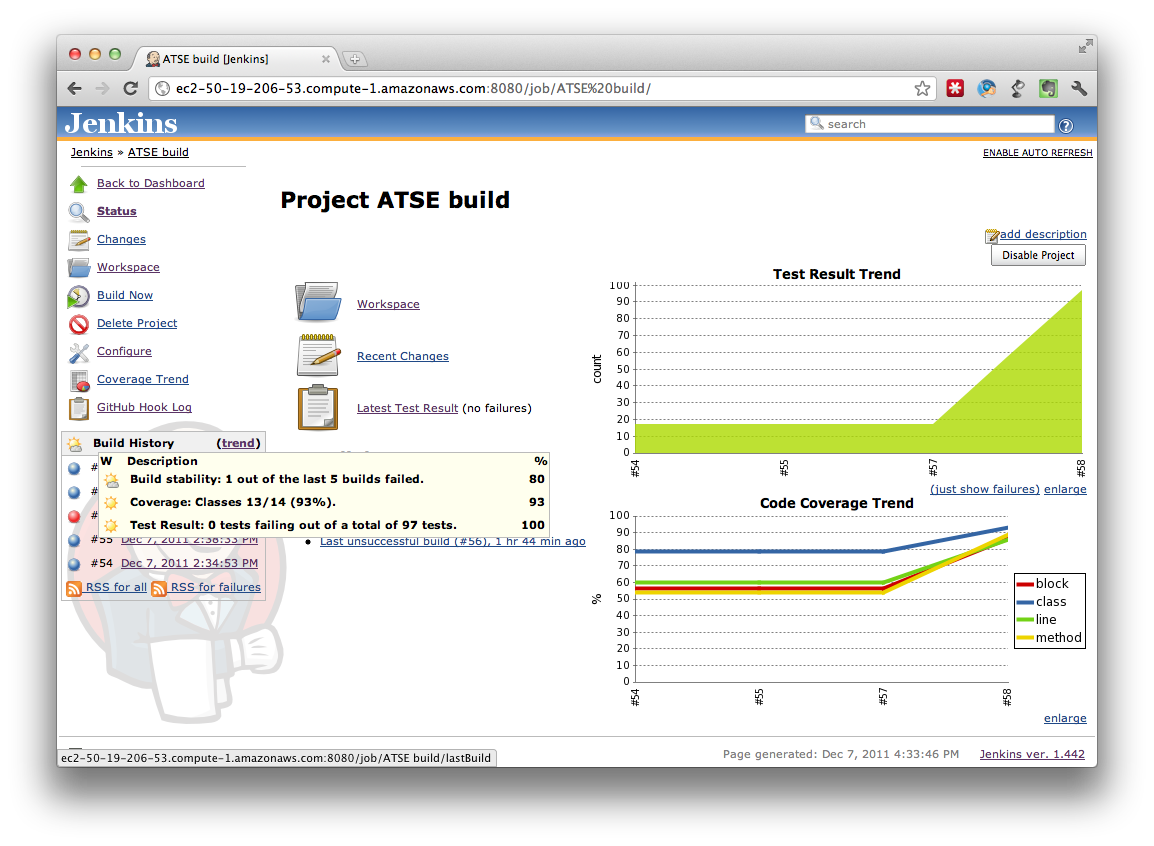
\includegraphics[scale=0.4]{images/jenkins_project.png}

%\section{Something else}
\pagebreak

% Managing future improvements
\section{Future Improvements}

Possible future improvements:
\begin{itemize}
\item As we have interface BillGenerator there is the possibility of implementing new styles of bill such as grouped bills or bills sorted in different ways. 
\item The interface CallLogger introduces the possibility of a Asynchronous call logger where you can be calling multiple people at the same time.
\item Define default charging behaviour for calls that last for a second, maybe there should be a minimum charge?
\item Extend call events to allow for more description of the calls, e.g hangup events and hold events.
\item Implementing a DSL to aid in constructing calls, extending that provided by JodaTime and Hamcrest
\item Implement port and adapters to add a layer of abstraction to the CustomerLibrary and Tariff to insulating from change and politics in other parts of the company
\end{itemize}

If these future improvements were to be added the same methodology could be used as it will scale as the 
number of developers and commits increases. That said, there are a number of improvements we would make. 
\\

\textbf{Infrastructure hosting}: The git repository would have to be hosted on its own server and builds would run much faster on faster machine(s) for Jenkins.

\textbf{Continuous Deployment}: See Development Processes

\textbf{Code Quality:} Jenkins picks up all the functional shortcomings of commits when it runs the various testing frameworks. Subjective matters such as code style and implementation details can't be vetted easily and having formal code review upon commit using a Jenkins plugin such as gerrit would be beneficial. This wasn't a problem as we were a small group with a small group so any bad code was picked noticed quickly. To ensure bad commits don't make it into the repository it would also be a good idea to use pre-tested commits where commits are tested and only committed to the repository if they pass.

\textbf{Registering issues:} If the system is under continued development it would make sense to record bugs and features to implement in an issue tracking and review system such as JIRA. JIRA manages the flow of issues as they get listed, get picked up by a developer, get implemented / fixed and then finally closed. 
Making these changes would ensure that the development of the system scales and the quality of the changes is high.


\end{document}